\documentclass[12pt]{tesislcc}

\begin{document}

\titulo{Clase y plantilla en \LaTeX \ para realizar una tesis de la Licenciatura en Ciencias de la 
Computación}
\autor{Julio Waissman Vilanova}
\director{Zutano Funánez Mengano}
\fecha{2016}

\frontcover

\frontmatter

\begin{summary}
En este apartado va un breve resumen del trabajo de tesis, de preferencia en media página en 
español y media página en inglés. Si no fuera el caso, pues una página a lo más en español. Es muy 
importante notar que el resumen no es una introducción. En el resumen no debe incluirse 
referencias bibliográficas ni listas. Mucha gente solo lee el resumen de un trabajo, así que es 
muy importante hacerlo muy cuidadosamente y que invite al que lo lee a seguir con el resto de la 
tesis. Esto es lo que se hace normalmente al último, cuando el resto de la tesis está acabada.
\end{summary}

\begin{dedication}
A la Virgencita de Guadalupe y el Santo Enmascarado de Plata
\end{dedication}

\begin{acknowledgements}
Esta sección se realiza al último, y una vez que se haya liberado la
tesis para su impresión. Los agradecimientos son completamente libres y pueden ser tan 
sentimentales, graciosos o profundos como se quiera. A diferencia de la dedicatoria, que debe 
caber en una sola línea, aquí se le puede agradecer hasta al perro si se les da la gana. Los 
agradecimientos no los revisa el director de tesis y por lo tanto no puede exigir que se incluyan 
agradecimientos a una u otra
persona en particular.

Igualmente, es importante resaltar que los agradecimientos y la
dedicatoria son completamente accesorios y si no se tiene la intención de agradecer a nadie (o no 
se quiere dedicar el trabajo a alguien), pues simplemente se eliminan y no hay ningún problema.
\end{acknowledgements}

\tableofcontents

\mainmatter

\introduccion
\xsection{Descripción del trabajo}

En la introducción es muy importante dejar claro cual era la
problemática a tratar, la justificación de dicho trabajo, los
objetivos (general y específicos) así como las metas. También es
importante acotar los alcances del trabajo. Esta información ya se
tiene del proyecto de tesis que se presentó antes de la realización de
la tesis, aunque en muchos casos es necesario adaptarla a lo que se
hizo realmente.

En un trabajo de tesis no es extraño empezar con un objetivo inicial y
conforme se desarrolla el trabajo derivar a otro problema o acotar el
problema original. Si este es el caso, es conveniente dejar claro en
la introducción de la tesis los objetivos, metas, justificación y
descripción \emph{del trabajo que se está presentando}.

Este capítulo no es muy largo y se escribe más fácilmente después de
escribir los capítulos del cuerpo de la tesis. Las secciones
siguientes (aportaciones principales y organización del trabajo)
suelen ser muy cortas (un párrafo o dos).

\xsection{Aportaciones principales}

Es una buena idea dejar en claro cuales son las aportaciones del
trabajo desde el principio. En este apartado se puede especificar
cuales son los trabajos, programas, publicaciones, prototipos o
revisiones realizadas. Así, se facilita la tarea del comité revisor y
facilita la lectura para quienes estén interesados en leer el trabajo.

Recuerda que es una tesis de licenciatura, y el hecho de estudiar un
artículo (o una técnica no vista durante la carrera), desmenuzarlo,
entenderlo, explicarlo y/o programarlo es suficiente. En una tesis de
licenciatra no se espera que se realice una aportación original.

\xsection{Organización del trabajo}

Facilita la lectura del trabajo describir que es lo que se presenta en el capitulo uno,
capitulo dos, etc. así como cuales son los apéndices que se agregan
al trabajo de tesis.


\chapter{Un primer capítulo}
\section{Introducción}

Es una buena costumbre comenzar cada capítulo con una sección de
introducción donde se describa lo que se va a mostrar en este
capítulo. Es más fácil escribir esta sección después de haber escrito
el capítulo completo. En este capítulo se introducen las ideas
generales para escribir un trabajo de tesis y su organización,
pensando en un trabajo de la Licenciatura en Ciencias de la
Computación de la Universidad de Sonora.

 \section{¿Como se organiza una tesis?}

 \subsection{Numero de capítulos}

 ¿Cuantos capítulos son necesarios para una tesis? Esto varía mucho
 dependiendo de la forma en que está organizado el trabajo, en común
 acuerdo con el director de tesis. Normalmente es mejor poner uno o
 dos capítulos que describan el estado del arte, las técnicas o las
 bases teóricas del trabajo a realizar, y que se utilizarán en el
 resto de la tesis.  En estos capítulos no se presentan ideas nuevas
 ni el desarrollo que más costó trabajo, solo las bases necesarias
 para entender el trabajo realizado. Se puede considerar una especie
 de revisión bibliográfica y suelen tener la mayor parte de las
 referencias bibliográficas de todo el trabajo escrito.

 En los capítulos subsecuentes, lo normal es ser muy específico y
 desarrollar con detalle el trabajo realizado, tanto si es un
 desarrollo teórico, un desarrollo tecnológico, como si es simulación
 o experimentación real. Estos capítulos suelen ser relativamente
 cortos y con muchas imágenes, gráficas y tablas en el caso de
 trabajos aplicados.

 Es común que una tesis de licenciatura tenga 3 capítulos, sin contar
 el capítulo de introducción y las conclusiones generales. Es importante resaltar que esto
 depende mucho de la naturaleza del trabajo desarrollado y debe ser
 establecido de antemano en común acuerdo entre el director de tesis y
 el estudiante. Igualmente, cabe resaltar que es normal, durante el
 desarrollo de la tesis (y más específicamente durante su redacción)
 que se considere agregar y/o quitar capítulos sobre el proyecto
 original.

 \subsection{¿Y la cantidad de páginas de una tesis?}

 ¿Cuantas cuartillas debe tener una tesis? Es una pregunta muy normal
 que se hacen todo mundo cuando comienza la fase de redacción. Las
 páginas correctas son \emph{las que sean necesarias para explicar el
   trabajo desarrollado}. Este número cambia mucho dependiendo de la
 disciplina. Por ejemplo, los trabajos en computación teóricas suelen
 ser muy cortos (unas 30 páginas para una tesis de licenciatura),
 mientras los trabajos enfocados a ingeniería de \emph{software}
 tienden a ser muy extensos (de 80 a 100 páginas).

 Es recomendable hacer un trabajo breve, normalmente entre 30 y 50
 páginas. Sin embargo, no existe una limitante, si el trabajo, por su
 naturaleza, requiere que sea explicado en más espacio, o naturalmente
 se tiende a escribir mucho. Se puede extender el trabajo de tesis
 \emph{hasta 100 páginas como máximo}. Es importante tomar en cuenta que en
 muchas Universidades del mundo, se tiende a limitar los trabajos de
 tesis de doctorado a 150 páginas como máximo con todo y apéndices. Un
 trabajo muy largo no significa que sea mejor.


 \subsection{¿Y como organizar el trabajo?}

 Para organizar el trabajo, \LaTeX contempla el uso de
 \verb+\section+, \verb+\subsection+, \verb+\subsubsection+ y
 \verb+\paragraph+. Si bien en este capítulo se hace uso de la mayoría
 de estos bloques con fines ilustrativos, en general es mejor tratar
 de mantener la organización del trabajo hasta
 \verb+\subsection+. Considere el uso de listas, enumeraciones y
 descripciones si requiere escribir muchos párrafos cortos con títulos
 en \verb+\subsubsection+ o \verb+\paragraph+. Igualmente, evite el
 uso excesivo de listas en un trabajo, ya que esto solo denota una
 pobre capacidad para expresar ideas en párrafos de texto.


 \section{Escribir un trabajo en \LaTeX}


Para realizar un trabajo científico en el área de Ciencias de la
Computación, especialmente en las ramas de computación teórica,
computo científico e inteligencia artificial, es normal utilizar
\LaTeX. Se asume que es normal que un estudiante que está preparando
una tesis de licenciatura en Ciencias de la Computación tenga
experiencia previa en escribir trabajos más pequeños en \LaTeX. 

Un buen comienzo para escribir un trabajo en \LaTeX, es buscar en otros trabajos un
ejemplo de algo similar a lo que queremos hacer, y luego adaptarlo a
las necesidades particulares. Por esta razón, en esta sección se
incluyen ejemplos para la inserción de figuras, cuadros, listas y
descripciones. Utilice estas plantillas, pero tenga cuidado en su
uso. Un problema muy común es el copiar la plantilla para la inserción
de figuras o cuadros, sin cambiar el comando \verb+\label+, por lo que
a la hora de compilar, se hace referencia en todo el documento a una
sola imagen.


\subsection{Inserción de figuras}


Las imágenes soportadas en la clase (y compiladas con \verb+pdflatex+)
son PNG, JPG, GIF y PDF de preferencia. Evitar utilizar imágenes de
tipo EPS. La figura \ref{fig:pdf} es un ejemplo de inserción de un
gráfico en PDF. La figura \ref{fig:png} y la figura \ref{fig:jpg} son
ejemplo para insertar imagenes en PNG y JPG respectivamente. La
leyenda de las figuras \emph{siempre} se encuentra por abajo de la
figura o imagen. 

\begin{figure}[tb!]
	\centering
    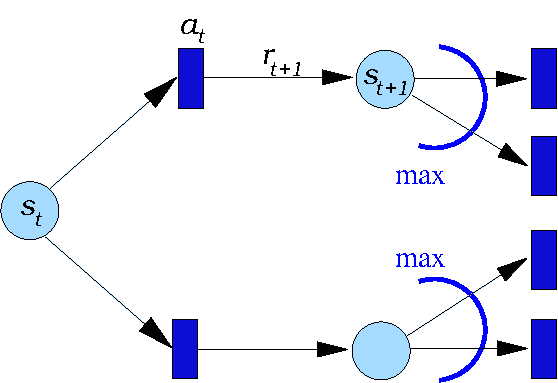
\includegraphics[width=0.5\textwidth]{tesislcc/ejemplo1.pdf}
    \caption{Ejemplo de inserción de una imagen en PDF}
    \label{fig:pdf}
\end{figure}

\begin{figure}[htb!]
	\centering
    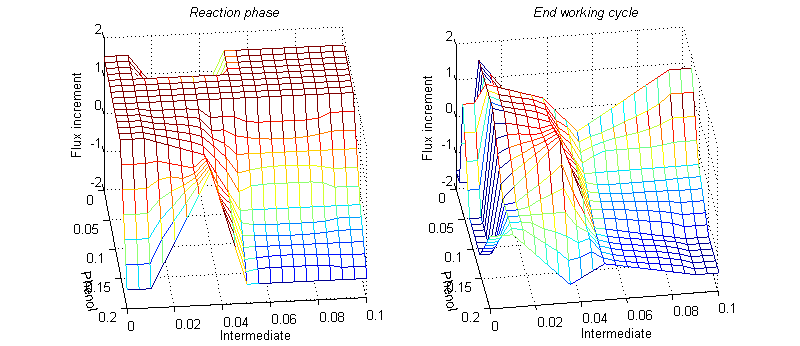
\includegraphics[width=0.7\textwidth]{tesislcc/ejemplo2.png}
    \caption{La leyenda de la figura siempre va abajo de ésta}
    \label{fig:png}
\end{figure}

\begin{figure}[htb!]
	\centering
    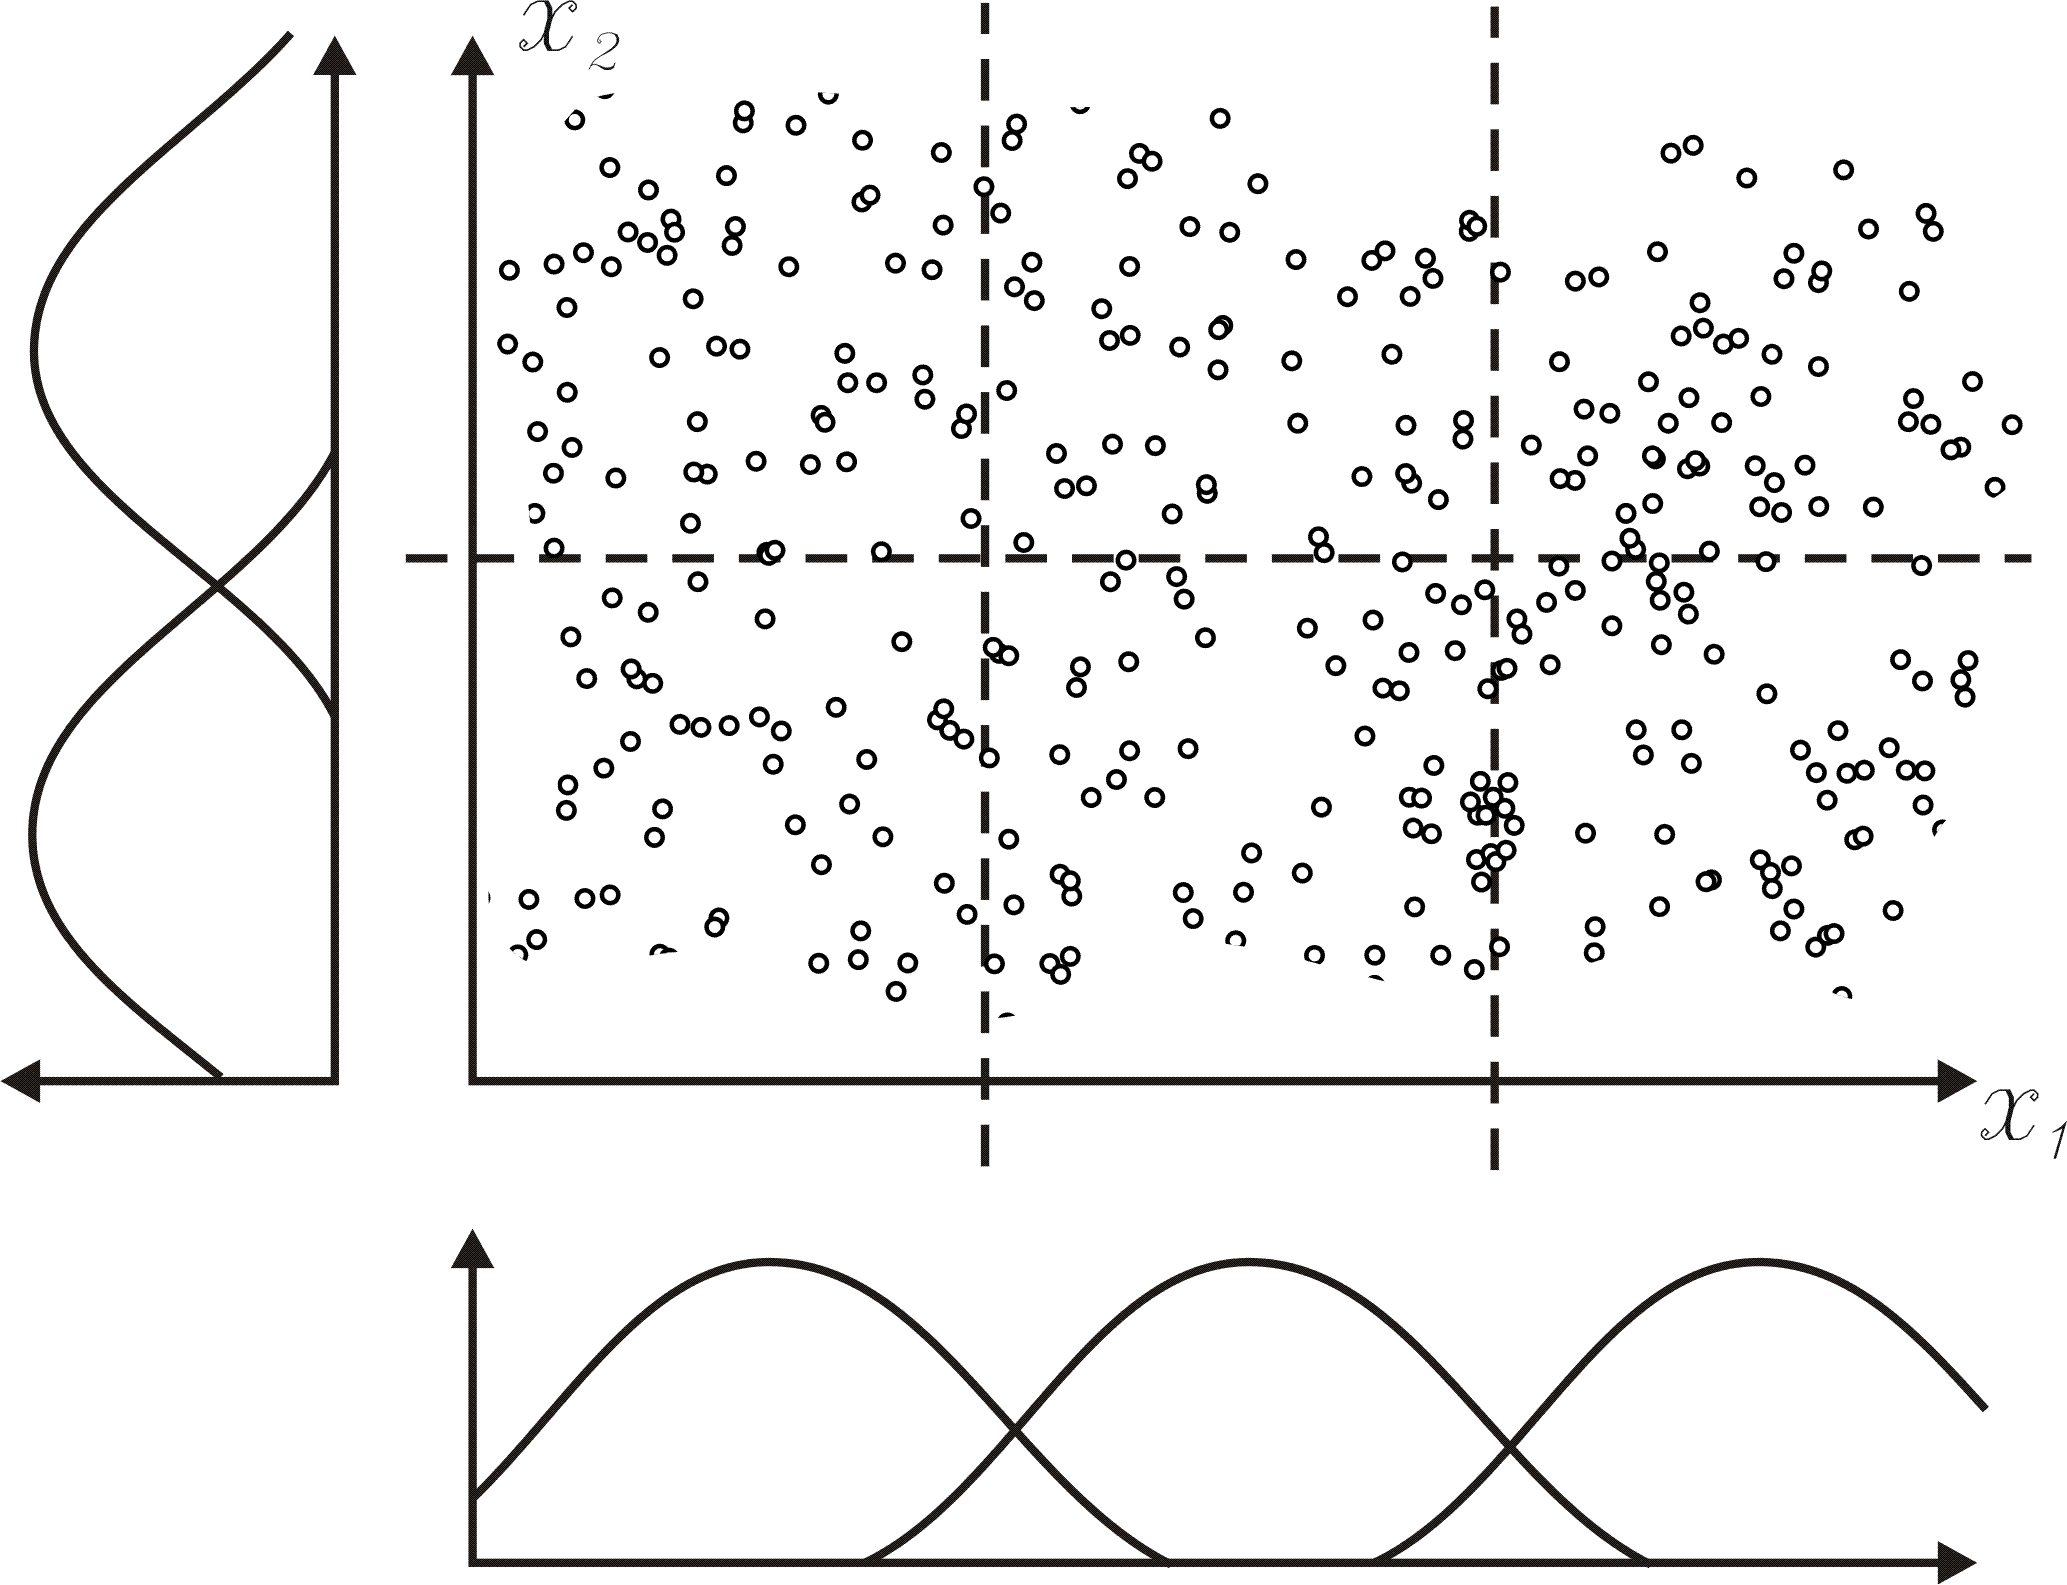
\includegraphics[width=0.5\textwidth]{tesislcc/ejemplo3.jpg}
    \caption{Procure que la leyenda explique claramente el
        título de la figura, aunque sea necesario que sea una leyenda
        larga que ocupe varias líneas}
    \label{fig:jpg}
\end{figure}


La colocación de una figura se puede controlar con los commandos
\texttt{h,t,b,p} (de \emph{here},\emph{top},\emph{bottom},\emph{page})
utilizando el orden como prioridad. Si por alguna extraña razón se
desea colocar una figura en un lugar específico del texto, se coloca
con el comando \texttt{H} (\emph{here} pero mandatorio). En general (y
esto es tanto para las tablas como para las figuras) no debe mucho
preocupar si las figuras se colocan en páginas diferentes que en las
que se hace referencia de ellas. 

Editorialmente esto es válido y recomendable. \LaTeX \ lo
que intenta es colocar las figuras siempre arriba de una página y evitar que el
porcentaje de texto en una página sea menor al 30\% de su contenido.
En la clase de tesis\verb+tesislcc+ se amplió el margen para
poder colocar figuras mas grandes, o varias figuras en una página. 

Es muy importante que se haga
referencia de todas las figuras en el texto y se discuta sobre ellas,
así sea sólo una línea de texto. Si no es posible hacer referencia de
una figura en el texto, significa que no es necesario que se encuentre
en el documento.

Otra práctica común y que suele ayudar mucho, sobre todo cuando la
tesis se encuentra bastante avanzada o cuando se piden cambios por
parte de los revisores, es el utilizar uno o varios directorios en los cuales se guarden las
figuras. Esto es especialmente importante en trabajos experimentales o
de desarrollo tecnológico que típicamente llevan varias capturas de
pantallas o muchas gráficas. En este ejemplo, las figuras se
encuentran agrupadas en un subdirectorio \texttt{figuras} (haciendo
gala de falta de imaginación).



\subsection{Inserción de cuadros}



Por abuso del idioma, tendemos a decirle en español tablas a lo que de
manera correcta deberíamos nombrar como \emph{cuadros}. Esto se debe a
que en inglés se les conoce como \emph{tables}. La leyenda de los
cuadros \emph{siempre} se encuentra arriba del cuadro (al revés que en las
figuras). El cuadro \ref{Ta:primer ejemplo} es un ejemplo típico de
cuadro. Es importante siempre citar y explicar un cuadro en el texto,
de otra manera significa que no es una información  necesaria. 


\begin{table}
  \centering
  \caption{Tabla de muestra para la tesis}
  \label{Ta:primer ejemplo}
  \vspace{.1cm}
  
  \begin{tabular}{|l|c|r|}
    \hline
    % after \\: \hline or \cline{col1-col2} \cline{col3-col4} ...
    Texto & Formulas & Numero \\
    \hline\hline
    Cosa & $\sqrt{x^2 + b^2}$ & 3.1416 \\
    Pasto & $3.2 + e^{-t}$ & 4578 \\
    \hline
  \end{tabular}
\end{table}

Todas las referencias (a figuras, cuadros, secciones, etc.) se deben
hacer utilizando los comandos \verb+label+ (para marcar un entorno) y
\verb+ref+ (para citarlo en el texto). En documentos muy grandes esto
es muy importante, ya que si se elimina o se agrega un cuadro o
figura, no es necesario reescribir todo el texto y revisar que se
haga referencia correcta de ellos en el texto.



\subsection{Escribiendo matemáticas}


Todos los estudiantes que realizan una tesis y requieren
de formalismo matemático, en general escogen \LaTeX como entorno de edición
preferencialmente, ya que la calidad tipográfica, como la facilidad
para incluir notación matematica en el texto, hacen que, en términos
generales, sea mucho más fácil escribir una tesis en \LaTeX que en un
entorno tipo WYSIWYG como \emph{World}. En esta sección se asume que
el lector se encuentra familiarizado con el uso de \LaTeX y el uso de
notación matemática, por lo que solamente se realizarán pequeñas recomendaciones. 





\section{Conclusiones}
En general, no es nada mala idea poner una última sección con
conclusiones de lo que se mostró en el capítulo. Para los revisores
y/o lectores del trabajo, les facilita mucho realizar una primer
hojeada al documento.

%%% Local Variables: 
%%% mode: latex
%%% TeX-master: "Tesis"
%%% End: 


\chapter{Otro capítulo de ejemplo}
\section{Introducción}

 En todo trabajo es normal comenzar cada capítulo con una sección de
 introducción donde se describa lo que se va a mostrar en este
 capitulo.Como en la tesis, es más fácil hacer esta sección al final
 del capitulo.

 \section{Que poner}

 \subsection{Numero de capítulos}

 Los capítulos que sean necesarios.Normalmente es mejor poner
 capítulos que describan el estado del arte, y las bases de lo que
 se usó en el desarrollo de la tesis. En estos capítulos, no se
 presentan ideas nuevas o desarrollos propios, solo lo que ya
 estaba. Es una especie de revisión bibliográfica.

 En los capítulos subsecuentes, lo normal es ser muy específico y
 desarrollar con detalle el trabajo realizado, tanto si es
 desarrollo tecnológico como si es en simulación o en experimentación
 real. Estos capítulos suelen ser relativamente cortos y con muchas
 imágenes, gráficas y tablas.

 \subsection{Otras cosas}

 Para poner cosas es bueno basarse en formatos ya preestablecidos.
 La notación de las tablas va antes de la tabla, mientras que la de
 las figuras va abajo. Siempre que se muestra una figura o una tabla
 hay que comentarla en el texto tal como la tabla (\ref{Ta:primer ejemplo2})



\begin{table}
  \centering
  \caption{Tabla de muestra para la tesis}
  \label{Ta:primer ejemplo2}
  \begin{tabular}{|l|c|r|}
    \hline
    % after \\: \hline or \cline{col1-col2} \cline{col3-col4} ...
    Texto & Formulas & Numero \\
    \hline\hline
    Cosa & $\sqrt{x^2 + b^2}$ & 3.1416 \\
    Pasto & $3.2 + e^{-t}$ & 4578 \\
    \hline
  \end{tabular}
\end{table}


\subsection{Mas cosas pa poner}

Pues en este caso solo se agrega una figura. Es importante ver que
para que el documento se mantenga ordenado se ponen las figuras en
un subdirectorio figuras y se llaman desde ahí.

\begin{figure}
	\centering
	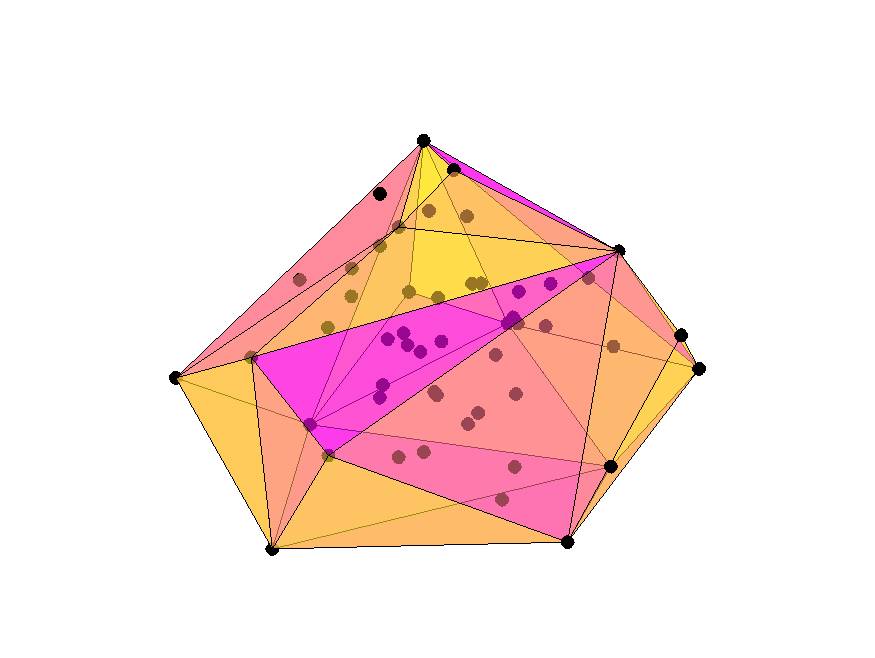
\includegraphics[width=.7\textwidth]{tesislcc/tesela.pdf}
    \caption{Ejemplo de una figura pa la tesis}
    \label{fig:teselacion}
\end{figure}

y bueno pues con esto creo que vemos en general como hacerle en
grandes lineas.

\section{Conclusiones}
En algunos casos no es nada mala idea poner una última sección con
conclusiones de lo que se mostró en el capítulo. 


\chapter{Citas y algoritmos}
\section{Introducción}

En este capítulo se abordará la manera agregar citas de la bibliografía; referencias a figuras y 
cuadros; algoritmos.\\

\section{Citas textuales y referencias}

En el documento se puede hacer referencia tanto a \emph{labels} (etiquetas) o entradas en la 
bibliografía.\\

\subsection{A figuras y cuadros}
En el caso de las referencias a figuras o cuadros se utiliza el comando \texttt{\textbackslash 
cref\{label\}}, en donde \texttt{label} es el nombre del identificador de la figura o tabla. Por 
ejemplo, en el \cref{Ta:primer ejemplo2} podemos observar que se ven unas fórmulas matemáticas 
chistosas.\\

\subsection{A la bibliografía}
En el caso de las referencias a entradas de la bibliografía se utiliza el comando 
\texttt{\textbackslash cite\{label\}}, en donde \texttt{label} es el nombre de la entrada de la 
referencia bibliográfica. Por ejemplo, el artículo de Sachdeva \cite{chackra} presenta una 
novedosa y arcana técnica para la regularización de los \emph{chakras}.\\

\subsection{Múltiples referencias}
En ocaciones es deseable referenciar a dos o mas etiquetas o entradas de la bibliografía, en dicho 
caso se pueden enlistar los argumentos de los comandos \texttt{\textbackslash cref} y 
\texttt{\textbackslash cite} separados por comas. Por ejemplo, dos trabajos de tesis que fueron 
inspiración para la elaboración de las \cref{fig:pdf,fig:png} fueron 
\cite{ejemplo_maestria,ejemplo_tesis_doctoral}.

\section{Códigos}

\subsection{Seudocódigos}
Para escribir algoritmos en seudocódigo con palabras clave en español podemos utilizar el entorno 
\texttt{algorithm} y \texttt{algorithmic}, el primero nos permite etiquetar y titular el 
algoritmo, mientras que el segundo es el entorno en donde se escribe el seudocódigo. Por ejemplo, 
el algoritmo \cref{alg1} describe la operación de potenciación.\\

\begin{algorithm}
	\caption{Calcula $y = x^n$}
    \label{alg1}
    \begin{algorithmic}
		\REQUIRE $n \geq 0 \vee x \neq 0$
        \ENSURE $y = x^n$
        
        \STATE $y \leftarrow 1$
        
        \IF{$n < 0$}
        	\STATE $X \leftarrow 1 / x$
            \STATE $N \leftarrow -n$
        \ELSE
        	\STATE $X \leftarrow x$
            \STATE $N \leftarrow n$
        \ENDIF
        
        \WHILE{$N \neq 0$}
        	\IF{$N$ es par}
            	\STATE $X \leftarrow X \times X$
                \STATE $N \leftarrow N / 2$
            \ELSE[$N$ es impar]
            	\STATE $y \leftarrow y \times X$
                \STATE $N \leftarrow N - 1$
            \ENDIF
        \ENDWHILE
	\end{algorithmic}
\end{algorithm}

Podemos tomar el ejemplo del algoritmo \emph{quicksort} del Cormen, el cual tiene un tiempo de 
ejecución en el peor de los casos de $\Theta \left(n^2 \right)$ y en el caso promedio $\Theta 
\left( n \lg n \right)$ sobre un arreglo de entrada de $n$ números y escribirlo de manera similar 
a como aparece en el libro \cref{alg:quicksort}.\\

\begin{algorithm}
	\caption{Ordenamiento \emph{quicksort}}
    \label{alg:quicksort}

	\vspace{10 pt}
	$\textsc{Quicksort}\left(A,p,r\right)$

    \begin{algorithmic}[1]
		\IF{$p < r$}
        	\STATE $q \leftarrow \textsc{Partition} \left( A, p, r \right)$
            \STATE $\textsc{Quicksort}\left( A, p, q-1 \right)$
            \STATE $\textsc{Quicksort}\left( A, q+1, r \right)$
        \ENDIF
	\end{algorithmic}
    
    \vspace{10 pt}
    $\textsc{Partition}\left(A,p,r\right)$
    \begin{algorithmic}[1]
    	\STATE $x \leftarrow A\left[r\right]$
        \STATE $i \leftarrow p-1$
        \FOR{$j\leftarrow p$ \TO $r-1$}
        	\IF{$A\left[j\right] \leq x$}
            	\STATE $i \leftarrow i+1$
                \STATE intercambia $A\left[i\right]$ con $A\left[j\right]$
            \ENDIF
        \ENDFOR
        \STATE intercambia $A\left[i+1\right]$ con $A\left[r\right]$
        \RETURN $i + 1$
    \end{algorithmic}
\end{algorithm}

\subsection{Códigos fuente}

Si el código que deseamos mostrar está escrito en algún lenguaje de programación en particular, 
utilizamos los entornos \texttt{listing} y \texttt{minted}. Por ejemplo, el 
\cref{code:rubyexample} es un ejemplo de código en el lenguaje \emph{Ruby}.\\

\begin{listing}[H]
\begin{minted}[frame=single]{ruby}
lazy_integers = (1..Float::INFINITY).lazy
lazy_integers.collect { |x| x ** 2 }.
              select { |x| x.even? }.
              reject { |x| x < 1000 }.
              first(5)
\end{minted}
\caption{Ejemplo de código en Ruby}
\label{code:rubyexample}
\end{listing}

El programa descrito en el \cref{code:helloworld} es todo un clásico en el mundo de la 
programación.\\

\begin{listing}[H]
\begin{minted}[frame=single]{c}
#include <stdio.h>

main()
{
    printf("hello, world\n");
}
\end{minted}
\caption{Clásigo \emph{hola mundo} en el lenguaje \emph{C}.}
\label{code:helloworld}
\end{listing}



\conclusiones
En las conclusiones no se separan por secciones, pero deben llevar
tres elementos básicos:
\begin{enumerate}
  \item Un breve resumen del trabajo realizado
  \item Un análisis critico de las ventajas y desventajes del
  trabajo realizado, procurando mostrar, al realizar una critica
  razonada de lo realizado, que se tiene un dominio del tema.
  \item Trabajos futuros derivados de lo realizado en esta tesis.
  Muchos de estos trabajos van a ser la solucion propuesta a los
  puntos débiles del trabajo realizado
\end{enumerate}

Las conclusiones pueden llevar más de una página, pero no es normal
encontrar conclusiones con una extensión mayor a las 3 páginas. En
este capitulo es muy importante ser muy claro y conciso. Típicamente
se realiza al final del trabajo y antes dehacer la introducción y el
resumen.


\appendix

\chapter{Información adicional}
\section{¿Porque poner apéndices?}

Hay cosas en una tesis que costaron mucho trabajo, que son
interesantes de mostrar para simplificar el trabajo de otras
personas que continúen con el trabajo realizado, pero que son áridos
de leer o no aportan mucho en el desarrollo del tema principal. En
ese caso los apéndices es la solución ideal para mostrarlos.

Este es el caso de los programas (código fuente) o bases matemáticas
de alguna técnica, en donde la aplicación es lo importante en el
trabajo de tesis. Por favor, incluye código fuente solo si es
extrictamente necesario, o si por la naturaleza del trabajo no se
puede
explicar con pseudocódigo. Es una tesis en Ciencias de la Computación
y se asume que todo el que la lee sabe programar. Un caso particular
donde el código es importante es cuando el trabajo se trata del uso de
una plataforma o una técnica muy específica (como podría ser
\emph{Jess}, o el uso de librerías para \emph{MPI}).

\section{Otros casos}

Otros casos importantes es donde es necesario poner a disposición la
información utilizada de otra fuente, tal como las bases de datos o
las bibliotecas de funciones realizadas por otras personas. Es común
en algunas tesis de agregar un último apéndices con los artículos
que se desarrollaron durante la tesis.


\listoffigures

\listoftables

\listofalgorithms

\listoflistings

\nocite{*}

\bibliografia{biblio}


\end{document}
